\chapter[Analiza problemu]{Analiza problemu}

\label{chapter:analiza_problemu}

% W tym rozdziale trzeba bardziej szczegółowo opisać jak chce Pan
% zrealizować cele sformułowane w rozdziale 2.
% Jakie będą konsekwencje i ewentualne wyzwania techniczne
% związane z przyjętą strategią. Jaka ogólnie ma być komunikacja
% z komputerem, tzn. czy to ma być tryb pytanie-odpowiedź, czy ciągłe
% przesyłanie danych. Czy być może jakiś tryb mieszany.
% Jaką chce Pan przyjąć formę przetwarzania danych i dlaczego. itd. itd.


\section{Generowanie i odbieranie sygnału ultradźwiękowego}

Od nadajnika wymaga się, by był zdolny do emitowania mocnego sygnału tylko dla jednej częstotliwości określonej w rozdziale \ref{chapter:przeglad_czujnikow}.
Do tego celu idealnie nadają się przetworniki piezoelektryczne o częstotliwości rezonansowej \unit[40]{kHz}. W celu zwiększenia wydajności takiego przetwornika,
konieczne jest podniesienie napięcia sygnału pobudzającego. Powinno zostać to zrealizowane za pomocą wzmacniacza prądowego oraz transformatora. 
Sterownik nadajnika musi pozwalać na wygenerowanie dokładnie określonej ilości impulsów. 
Mechanizm ten umożliwia urządzeniu wykonywać sekwencje odczytu o różnych parametrach, które mogą mieć wpływ na jakość danych wyjściowych. 
Ze względu na wybranie mikrofonu o bardzo szerokim paśmie przenoszenia, konieczne jest zastosowanie filtrów pasmowych. 
Muszą mieć one szczyt skuteczności w zakresie częstotliwości rezonansowej nadajnika, pozwoli to na rozróżnienie sygnału docelowego od innych zakłóceń oraz szumu tła.



\section{Określenie kierunku nadejścia odebranego sygnału}
W publikacji \cite{Kreczmer:2020:Azimuth:Elevation},
do wyznaczenia kierunku nadejścia sygnału została użyta metoda polegająca na pomiarze przesunięcia fazowego.
Może to być osiągnięte poprzez umieszczone na wspólnej powierzchni odbiorniki. 
Jeżeli odstępy pomiędzy mikrofonami są mniejsze niż pół długości fali odbieranego sygnału, 
to do pomiaru wystarczającą konfiguracją są trzy odbiorniki ustawione niewspółliniowo (patrz rys. \ref{fig:micarray}).
W przypadku gdy odległość między odbiornikami jest stosunkowo mała do odległości od wykrywanego obiektu , 
od którego odbity zostaje sygnał, fala dźwiękowa może być traktowana jako płaska powierzchnia. 
Zakładając, że $ t_0, t_1, t_2 $ to czasy, w których ta sama powierzchnia została wykryta odpowiednio przez odbiorniki $R_0, R_1$ i $R_2$, 
a jednocześnie $t_0 \leq t_1$ i $t_0 \leq t_2$, to odległości odbiorników $R_1$ i $R_2$ 
od powierzchni w momencie dotarcia do $R_0$ wynoszą następująco:

\begin{equation}
	s_1 = v_a\tau_{01}, \qquad s_2 = v_a\tau_{02},
\end{equation}

gdzie $v_a$ jest prędkością fali, $\tau_{01} = t_1-t_0$ i $\tau_{02} = t_2-t_0$. 
Ponieważ w uproszczonym modelu fala dźwiękowa jest płaską powierzchnią musi spełnić równanie:

\begin{equation}
	ax + by +cz+d = 0,
\end{equation}
gdzie $a, b$ i $c$ to koordynaty wektorów prostopadłych do powierzchni. Można założyć, że wektor jest znormalizowany i oznaczony jako $n = (n_x, n_y, n_z)$ oraz

\begin{equation}
	n_y^2 + n_z^2 + n_z^2 = 1.
\end{equation}

Do wyznaczenia kąta azymutu oraz elewacji obiektu można założyć, że wektor \textbf{n} jest skierowany przeciwnie 
do kierunku propagacji fali dźwiękowej. W tym przypadku oznacza to $n_x > 0$. Ponieważ wektor \textbf{n} jest znormalizowany, 
bezwzględna wartość $d$ jest odległością powierzchni od środka układu współrzędnych, 
który znajduję się w środku odbiornika $R_0$ (patrz rys. \ref{fig:micarray}).

\begin{figure}[ht!]
	\centering
	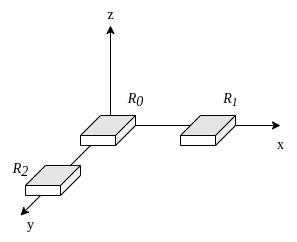
\includegraphics[width = 0.5\textwidth]{microphonearray.png}
	\caption{rozmieszczenie mikrofonów w przestrzeni trójwymiarowej}
	\label{fig:micarray}
\end{figure}


Biorąc pod uwagę poprzednie założenia oraz to, że koordynaty odbiorników $R_1$ i $R_2$ 
to odpowiednio $(0, y_1, z_1)$ i $(0, y_2, z_2)$ daje to układ równań:


\begin{equation}
	\begin{cases}
		n_y y_1 + n_z z_1 = s_1,\\
		n_y y_2 + n_z z_2 = s_2,\\
		n_y^2 + n_z^2 + n_z^2 = 1.	
	\end{cases}
\end{equation}
Rozwiązaniem tego układu równań jest:

\begin{equation}
	n_y= \frac{z_2s_1 - z_1s_2}{y_1z_2-y_2z_1},\qquad   n_z= \frac{y_1 s_2 - y_2 s_1}{y_1z_2-y_2 z_1}, \qquad  n_x= \sqrt{1-n_y^2-n_z^2}  
\end{equation}

\clearpage
Mając koordynaty znormalizowanego wektora, kąt azymutu $\Phi$ oraz elewację $\Theta$ można obliczyć za pomocą następujących równań:
\begin{align}
	&\Phi = arcsin \frac{n_y}{\sqrt{n_y^2 +n_x^2}}= arcsin \frac{n_y}{\sqrt{1-n_z^2}},\\
	&\Theta = arcsin \frac{n_z}{\sqrt{n_x^2+n_x^2}}= arcsin \frac{n_z}{\sqrt{1-n_y^2}}.	
\end{align}





% \begin{figure}[ht!]
% 	\centering
% 	\subfloat[]{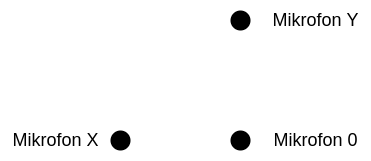
\includegraphics[width = 0.5\textwidth]{rozmieszczenie_mic.drawio.png}}
% 	\subfloat[]{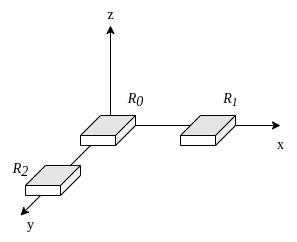
\includegraphics[width = 0.5\textwidth]{microphonearray.png}}
% 	\caption{Rozmieszczenie mikrofonów w przestrzeni: dwu wymiarowej a) oraz trój wymiarowej b)}
% 	\label{fig:micarray}
% 	  \end{figure}

\section{Komunikacja}
Komunikacja komputera typu PC z płytką deweloperską STM32 NUCLEO-L476RG, 
na której bazowany jest projekt odbędzie się przy pomocy portu szeregowego. 
Nowoczesne komputery są wyposażone w złącze USB, które ma niezwykły wpływ na standaryzację interfejsów w urządzeniach użytkowych. 
Większość płytek deweloperskich również posiada wbudowane gniazdo USB z portem szeregowym, 
Dlatego też wybór tego rodzaju komunikacji wydaje się wręcz oczywistą decyzją.
Tym samym złączem wgrywany jest również program do pamięci mikrokontrolera, co jeszcze bardziej upraszcza stanowisko testowe.
Dane będą wysyłane w postaci tekstu w formie pytanie-odpowiedź, 
gwarantując większą elastyczność i możliwość zmiany parametrów urządzenia przez użytkownika bez konieczności przeprogramowywania mikrokontrolera.
Jednocześnie to rozwiązanie nie spowoduje obniżenia efektywności komunikacji urządzenia z komputerem. 



